\chapter{循环}

\section{while}

\subsection{while}

在while循环中,当条件满足时重复循环体内的语句。如果条件永远为真,循环会永无止境的进行下去(死循环),因此循环体内要有改变条件的机会。\\

控制循环次数的方法就是设置循环变量:初值、判断、更新。\\

while循环的特点是先判断、再执行,所以循环体有可能会进入一次或多次,也有可能一次也不会进入。

\vspace{-0.5cm}

\begin{lstlisting}[language=C]
while(条件)
{
    // code
}
\end{lstlisting}

\vspace{0.5cm}

\mybox{计算5个人的平均身高}

\begin{lstlisting}[language=C]
#include <stdio.h>

int main()
{
    double height;
    double total = 0;
    double average;
    int i = 1;

    while(i <= 5)
    {
        printf("输入第%d个人的身高:", i);
        scanf("%lf", &height);
        total += height;
        i++;
    }

    average = total / 5;
    printf("平均身高:%.2f\n", average);  
    return 0;
}
\end{lstlisting}

\begin{tcolorbox}
	\mybox{运行结果}
	\begin{verbatim}
输入第1个人的身高:160.8
输入第2个人的身高:175.2
输入第3个人的身高:171.2
输入第4个人的身高:181.3
输入第5个人的身高:164
平均身高:170.5
\end{verbatim}
\end{tcolorbox}

\vspace{0.5cm}

\mybox{计算元音、辅音个数}

\begin{lstlisting}[language=C]
#include <stdio.h>

int main()
{
    char c;
    int vowel = 0;
    int consonant = 0;

    printf("输入一句英语句子:");

    while((c = getchar()) != '\n')
    {
        if(c == 'a' || c == 'e' || c == 'i' || c == 'o' || c == 'u' 
        || c == 'A' || c == 'E' || c == 'I' || c == 'O' || c == 'U')
        {
            vowel++;
        }
        else if((c >= 'a' && c <= 'z') || (c >= 'A' && c <= 'Z'))
        {
            consonant++;
        }
    }

    printf("元音 = %d\n", vowel);
    printf("辅音 = %d\n", consonant);
    return 0;
}
\end{lstlisting}

\begin{tcolorbox}
	\mybox{运行结果}
	\begin{verbatim}
输入一句英语句子:Hello World
元音 = 3
辅音 = 7
\end{verbatim}
\end{tcolorbox}

\newpage

\section{do-while}

\subsection{do-while}

do-while循环在进入循环的时候不做检查,而是在执行完一轮循环体的代码之后,再来检查循环的条件是否满足,如果满足则继续下一轮循环,不满足则结束循环,即至少执行一次循环。\\

do-while循环的主要特点是先执行、再判断。

\vspace{-0.5cm}

\begin{lstlisting}[language=C]
do {
    // code
} while(条件);
\end{lstlisting}

\vspace{0.5cm}

\mybox{计算整数位数}

\begin{lstlisting}[language=C]
#include <stdio.h>

int main() {
    int num;
    int n = 0;

    printf("输入整数:");
    scanf("%d", &num);

    do {
        num /= 10;
        n++;
    } while(num != 0);

    printf("位数:%d\n", n);
    return 0;
}
\end{lstlisting}

\begin{tcolorbox}
	\mybox{运行结果}
	\begin{verbatim}
输入整数:123
位数:3
\end{verbatim}
\end{tcolorbox}

\vspace{0.5cm}

\subsection{while与do-while区别}

while循环与do-while循环有以下区别:

\begin{enumerate}
	\item 执行顺序不同。

	\item 初始情况不满足循环条件时,while循环一次都不会执行,do-while循环不管任何情况都至少执行一次。

	\item do-while循环的while语句后有【;】。
\end{enumerate}

\begin{figure}[H]
	\centering
	
\includegraphics[scale=0.15]{img/C4/4-3/1.png}
\end{figure}

\vspace{0.5cm}

\mybox{猜数字}

\begin{lstlisting}[language=C]
#include <stdio.h>
#include <stdlib.h>     // 标准库
#include <time.h>

int main() {
    srand(time(NULL));          // 时间种子
    int answer = rand() % 100 + 1;  // 产生1-100之前的随机数
    int num = 0;
    int cnt = 0;

    do {
        printf("猜一个1-100之间的数字:");
        scanf("%d", &num);
        cnt++;
        
        if(num > answer) {
            printf("猜大了\n");
        } else if(num < answer) {
            printf("猜小了\n");
        }
    } while(num != answer);
    
    printf("猜对了!你一共用了%d次猜对!\n", cnt);
    return 0;
}
\end{lstlisting}

\begin{tcolorbox}
	\mybox{运行结果}
	\begin{verbatim}
猜一个1-100之间的数字:50
猜大了!
猜一个1-100之间的数字:25
猜小了!
猜一个1-100之间的数字:37
猜小了!
猜一个1-100之间的数字:43
猜小了!
猜一个1-100之间的数字:46
猜小了!
猜一个1-100之间的数字:48
猜小了!
猜一个1-100之间的数字:49
猜对了!你一共用了7次猜对!
\end{verbatim}
\end{tcolorbox}

\newpage

\section{for}

\subsection{for}

for循环有三个表达式,中间用【;】分隔,【;】不可省略。

\vspace{-0.5cm}

\begin{lstlisting}[language=C]
for(表达式1; 表达式2; 表达式3)
{
    //code
}
\end{lstlisting}

\begin{itemize}
	\item 表达式1通常是为循环变量赋初值,可省略。
	\item 表达式2是循环条件,判断是否继续执行循环,可省略。
	\item 表达式3为更新循环变量的值,可省略。
\end{itemize}

\vspace{0.5cm}

\mybox{计算1-100的累加和}

\begin{lstlisting}[language=C]
#include <stdio.h>

int main()
{
    int sum = 0;
    for(int i = 1; i <= 100; i++)
    {
        sum += i;
    }
    printf("%d\n", sum);
    return 0;
}
\end{lstlisting}

\begin{tcolorbox}
	\mybox{运行结果}
	\begin{verbatim}
5050
\end{verbatim}
\end{tcolorbox}

\vspace{0.5cm}

\mybox{计算$ 1 + {1 \over 2} + {1 \over 3} + ... + {1 \over n} $}

\begin{lstlisting}[language=C]
#include <stdio.h>

int main()
{
    int n;
    double sum = 0.0;
    printf("输入n:");
    scanf("%d", &n);

    for(int i = 1; i <= n; i++)
    {
        sum += 1.0 / i;
    }
    printf("%f\n", sum);
    return 0;
}
\end{lstlisting}

\begin{tcolorbox}
	\mybox{运行结果}
	\begin{verbatim}
输入n:10
2.928968
\end{verbatim}
\end{tcolorbox}

\vspace{0.5cm}

\mybox{斐波那契数列}

\begin{figure}[H]
	\centering
	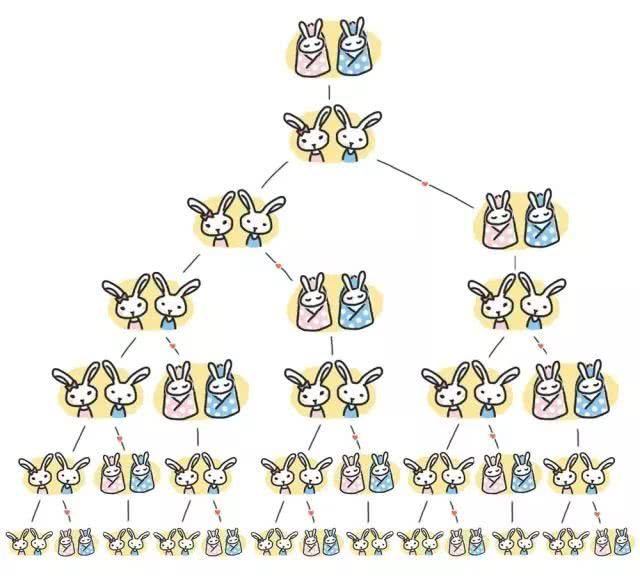
\includegraphics[scale=0.3]{img/C4/4-4/1.png}
\end{figure}

\begin{lstlisting}[language=C]
#include <stdio.h>

int main()
{
    int n;
    int num1, num2, val;

    printf("输入斐波那契数列长度:");
    scanf("%d", &n);

    if(n == 1)
    {
        printf("1\n");
    }
    else if(n == 2)
    {
        printf("1, 1\n");
    }
    else
    {
        num1 = 1;
        num2 = 1;
        printf("1, 1");
        for(int i = 3; i <= n; i++)
        {
            val = num1 + num2;
            printf(", %d", val);
            num1 = num2;
            num2 = val;
        }
        printf("\n");
    }
    return 0;
}
\end{lstlisting}

\begin{tcolorbox}
	\mybox{运行结果}
	\begin{verbatim}
输入斐波那契数列长度:10
1, 1, 2, 3, 5, 8, 13, 21, 34, 55
\end{verbatim}
\end{tcolorbox}

\vspace{0.5cm}

\subsection{嵌套循环}

循环也可以进行嵌套使用。\\

\mybox{九九乘法表}\\

\begin{table}[H]
	\centering
	\setlength{\tabcolsep}{1.5mm}{
		\begin{tabular}{|c|c|c|c|c|c|c|c|c|}
			\hline
			1*1=1 & 1*2=2  & 1*3=3  & 1*4=4  & 1*5=5  & 1*6=6  & 1*7=7  & 1*8=8  & 1*9=9  \\
			\hline
			2*1=2 & 2*2=4  & 2*3=6  & 2*4=8  & 2*5=10 & 2*6=12 & 2*7=14 & 2*8=16 & 2*9=18 \\
			\hline
			3*1=3 & 3*2=6  & 3*3=9  & 3*4=12 & 3*5=15 & 3*6=18 & 3*7=21 & 3*8=24 & 3*9=27 \\
			\hline
			4*1=4 & 4*2=8  & 4*3=12 & 4*4=16 & 4*5=20 & 4*6=24 & 4*7=28 & 4*8=32 & 4*9=36 \\
			\hline
			5*1=5 & 5*2=10 & 5*3=15 & 5*4=20 & 5*5=25 & 5*6=30 & 5*7=35 & 5*8=40 & 5*9=45 \\
			\hline
			6*1=6 & 6*2=12 & 6*3=18 & 6*4=24 & 6*5=30 & 6*6=36 & 6*7=42 & 6*8=48 & 6*9=54 \\
			\hline
			7*1=7 & 7*2=14 & 7*3=21 & 7*4=28 & 7*5=35 & 7*6=42 & 7*7=49 & 7*8=56 & 7*9=63 \\
			\hline
			8*1=8 & 8*2=16 & 8*3=24 & 8*4=32 & 8*5=40 & 8*6=48 & 8*7=56 & 8*8=64 & 8*9=72 \\
			\hline
			9*1=9 & 9*2=18 & 9*3=27 & 9*4=36 & 9*5=45 & 9*6=54 & 9*7=63 & 9*8=72 & 9*9=81 \\
			\hline
		\end{tabular}
	}
	\caption{九九乘法表}
\end{table}

\begin{lstlisting}[language=C]
#include <stdio.h>

int main()
{
    for(int i = 1; i <= 9; i++)
    {
        for(int j = 1; j <= 9; j++)
        {
            printf("%d*%d=%d\t", i, j, i*j);
        }
        printf("\n");
    }
    return 0;
}
\end{lstlisting}

\vspace{0.5cm}

\mybox{输出图案}

\begin{lstlisting}
*
**
***
****
*****
\end{lstlisting}

\begin{lstlisting}[language=C]
#include <stdio.h>

int main()
{
    for(int i = 1; i <= 5; i++)
    {
        for(int j = 1; j <= i; j++)
        {
            printf("*");
        }
        printf("\n");
    }
    return 0;
}
\end{lstlisting}

\newpage

\section{break or continue?}

\subsection{循环控制}

循环控制语句的作用是控制当前的循环结构是否继续向下执行,如果不进行控制,那么会根据既定的结构重复执行。如果有一些特殊的情况导致循环的执行中断,就称为循环的控制语句。循环控制语句的关键字有break和continue。\\

break的作用是跳出当前循环,执行当前循环之后的语句。break只能跳出一层循环,如果是嵌套循环,那么需要按照嵌套的层次,逐步使用break来跳出。break语句只能在循环体内和switch语句内使用。\\

continue的作用是跳过本轮循环,开始下一轮循环的条件判断。continue终止当前轮的循环过程,但它并不跳出循环。\\

\mybox{break}

\begin{lstlisting}[language=C]
#include <stdio.h>

int main()
{
    for(int i = 1; i <= 10; i++)
    {
        if(i == 5)
        {
            break;
        }
        printf("%d ", i);
    }
    return 0;
}
\end{lstlisting}

\begin{tcolorbox}
	\mybox{运行结果}
	\begin{verbatim}
1 2 3 4 
\end{verbatim}
\end{tcolorbox}

\vspace{0.5cm}

\mybox{continue}

\begin{lstlisting}[language=C]
#include <stdio.h>

int main()
{
    for(int i = 1; i <= 10; i++)
    {
        if(i == 5)
        {
            continue;
        }
        printf("%d ", i);
    }
    return 0;
}
\end{lstlisting}

\begin{tcolorbox}
	\mybox{运行结果}
	\begin{verbatim}
1 2 3 4 6 7 8 9 10 
\end{verbatim}
\end{tcolorbox}

\newpage